\subsection[SystemC Integration]{SystemC Integration}
\label{sec:systemc}

While the open and configurable architecture of gem5 is of particular interest
in academia, the industry's main tool for virtual prototyping is SystemC
Transaction Level Modeling (TLM)~\cite{systemc_ieee11}. Many hardware vendors
provide SystemC TLM models of their IP and there are tools, such as Synopsys
Platform Architect\footnote{\url{https://www.synopsys.com/verification/virtual-prototyping/platform-architect.html}},
that assist in building a virtual system and analyzing it. Also, many research
projects use SystemC TLM, as they benefit from the rich ecosystem of accurate
off-the-shelf models of real hardware components. However, there is a lack of
accurate and modifiable CPU models in SystemC since the model providers want to
protect their IP. This makes the combination of gem5 with SystemC very
attractive.

\subsubsection[gem5 to SystemC Bridge]{gem5 to SystemC Bridge\footnote{By Christian Menard, Matthias Jung, Abdul Mutaal Ahmad, and Jeronimo Castrillon}}

SystemC TLM and gem5 were developed around the same time and are based on
similar underlying ideas. As a consequence, the hardware model used by TLM is
surprisingly close to the model of gem5. In both approaches, the system is
organized as a set of components that communicate by exchanging data packets
via a well defined protocol. The protocol abstracts over the physical
connection wires that would be used in a register transfer level (RTL)
simulation and thereby significantly increases simulation speed. In gem5,
components use \emph{requestor} and \emph{responder} ports to communicate to other
components, whereas in SystemC TLM, connections are established via
\emph{initiator} and \emph{target} sockets. Also, the three protocols
\emph{atomic}, \emph{timing} and \emph{functional} provided by gem5 find their
equivalent in the \emph{blocking}, \emph{non-blocking} and \emph{debug}
protocols of TLM. The major difference in both protocols is the treatment of
backpressure, which is implemented by a retry phase in gem5 and with the
exclusion rule of TLM.

\begin{figure}
    \centering
    \subcaptionbox{gem5 to SystemC\label{fig:example:gem5_to_sc}}[.25\linewidth]{
      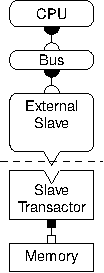
\includegraphics[height=4cm]{fig/gem5_to_systemc.pdf}
    }
    \subcaptionbox{SystemC to gem5\label{fig:example:sc_to_gem5}}[.25\linewidth]{
      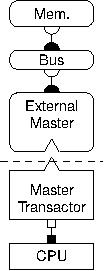
\includegraphics[height=4cm]{fig/systemc_to_gem5.pdf}
    }
    \subcaptionbox{both directions\label{fig:example:twoway}}[.25\linewidth]{
      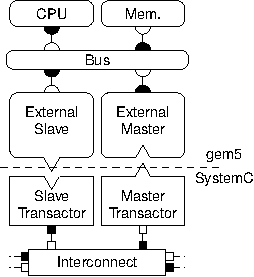
\includegraphics[height=4cm]{fig/twoway.pdf}
    }
    \caption{Possible scenarios for binding gem5 and SystemC.}
    \label{fig:gem5_tlm_example}
\end{figure}

The similarity of the two approaches enabled us to create a light-weight
compatibility layer. In our approach, co-simulation is achieved by hosting the
gem5 simulation on top of a SystemC simulation. For this, we replaced the gem5
discrete event kernel with a SystemC process that is managed by the SystemC
kernel. A set of transactors further enables communication between the two
simulation domains by translating between the two protocols as is shown in
Figure~\ref{fig:gem5_tlm_example}. Menard et al. documented our approach and showed
that the transaction between gem5 and TLM only introduces a low overhead of
about \(8\%\)~\cite{menard2017-system-systemc}.
The source code as well as basic usage examples can be found in
\texttt{util/tlm} of the gem5 repository.

\subsubsection[SystemC in gem5]{SystemC in gem5\footnote{By Gabriel Black}}

Alternatively, gem5 also has its own built in SystemC kernel and TLM implementation, and can run models natively as long as they are recompiled with gem5's SystemC header files.
These models can then use gem5's configuration mechanism and be controlled from Python, and, by using modified versions of the bridges developed to run gem5 within a SystemC simulation, TLM sockets can be connected to gem5's native ports.

This approach integrates models into gem5 more cleanly and fully since they are now first class gem5 models with access to all of gem5's APIs.
Existing models and \verb|c_main| implementations can generally be used as-is without any source level modifications; they just need to be recompiled against gem5's SystemC headers and linked into a gem5 binary.

While some parts of gem5's SystemC implementation are taken from the open source reference implementation (most of the data structure library and TLM), the core implementation is new and based off of the SystemC standard.
This means that code which depends on nonstandard features, behaviors, and implementation specific details of the reference implementation may not compile or work properly within gem5.
That said, gem5's SystemC kernel passes almost all of the reference implementation's test suite.
The few exceptions are tests that are broken, explicitly test for implementation specific behavior, or test for deprecated and undocumented features.
